%	$Id$
% Internal documentation for slide modeling in grdseamount
% Paul Wessel, November 16, 2016.
\documentclass[12pt,letterpaper,margin=0.5in]{report}
\usepackage{times}
\usepackage{graphicx}
\usepackage{breqn}
\usepackage[margin=0.5in]{geometry}
\usepackage{lscape}
\textheight = 9 in
\topmargin = -1 in
\begin{document}

\section{Modeling landslides in grdseamount}

\begin{figure}[h!]
  \centering
  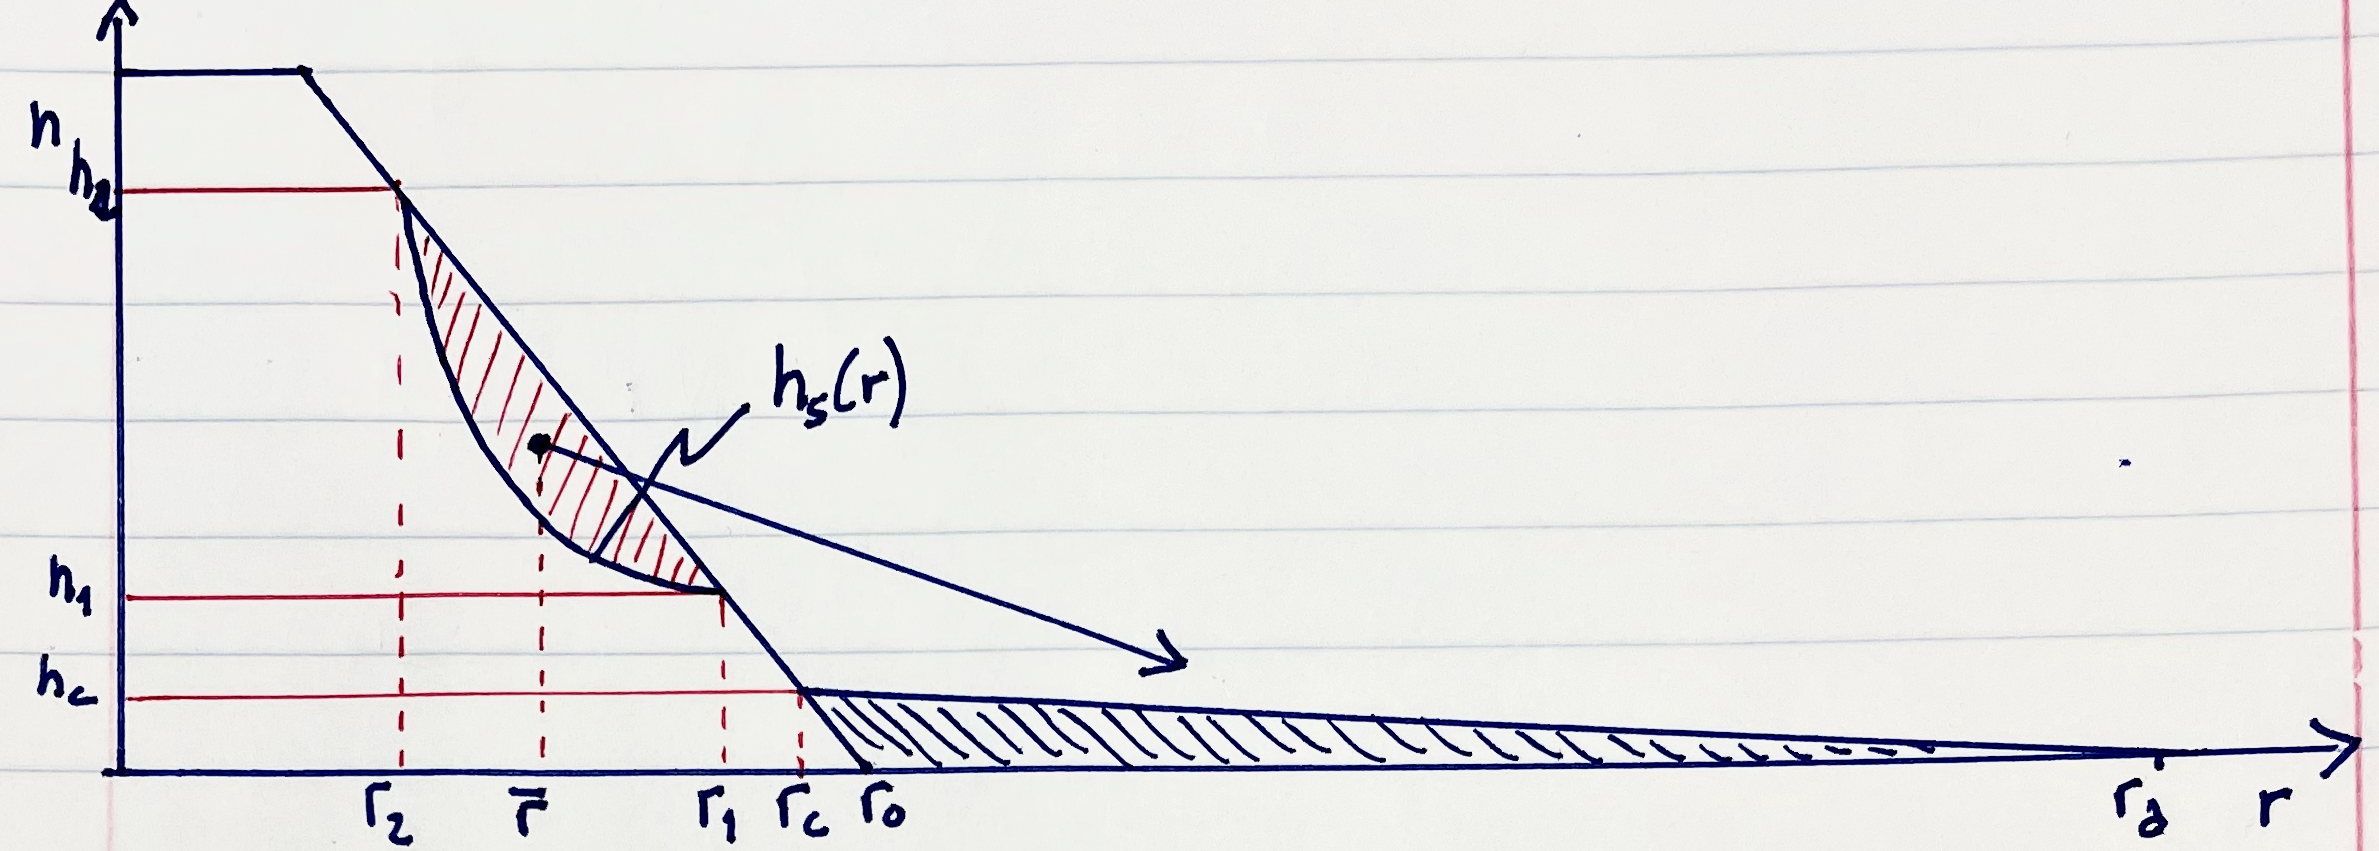
\includegraphics[width=5in]{slides_fig1.png}
  \caption{Geometry for an \emph{ad hoc} landslide approximation in \texttt{grdseamount}.  The slide material (pink)
  will be deposited at the toe of the seamount (light blue) starting at a height of $h_c$ and linearly
  tapering to zero at a distal point $r_d$. Note that $h_2 > h_1$ while $r_1 > r_2$.}
  \label{slides_fig1}
\end{figure}

We expand the work of {\it J. Smith and Wessel} (2000) on approximating large landslides off seamounts
for the purpose of studying the isostatic consequences of the mass redistribution (Figure~\ref{slides_fig1}).  The equation for the
cross-sectional shape of the slide for the radial range $r_2$ to $r_1$ is given by a single equation:
\begin{equation}
h_s(r) = h_1 + \Delta h \cdot q(u),
\end{equation}
where $\Delta h = h_2 - h_1$ is the \emph{height} range of the rupture surface and $q(u)$ is the normalized shape curve of the slide,
\begin{equation}
q(u) = u_0 \left (\frac{1 + u_0}{u + u_0} - 1 \right ),
\end{equation}
which is a hyperbolic curve. We use the tuning parameter $u_0$ to carve more or less deeply into the seamount core.
Here, $u$ is the normalized distance from $r_2$ to $r_1$, given by
\begin{equation}
u = \frac{r-r_2}{r_1 - r_2} = \frac{r-r_2}{\Delta r}, \quad \mbox{hence } r = r_2 + u \Delta r,
\end{equation}
where $\Delta r$ is the \emph{radial} range of the slide.
Figure~\ref{slides_fig2} shows typical shapes of $q(u)$ for some values of $u_0$.
\begin{figure}[h!]
  \centering
  \includegraphics[width=5in]{slides_fig2.png}
  \caption{A variety of slide shapes are possible by varying $u_0$.  The slide area for a conical seamount would be the area
  between the flank (dashed line) and the selected curve.}
  \label{slides_fig2}
\end{figure}

Depending on the shape of the seamount prior to the slide event (called $h(r)$, with $h_s(r) \le h(r)$), we will need to compute the various radii referred
to in Figure \ref{slides_fig1}, such as $r_1$, $r_2$, $r_c$, and $r_d$ from their corresponding heights $h_1$, $h_2$, $h_c$ and volume of slide.
The material removed by the land slide (pink)
will be deposited at the base of the seamount (light blue) starting from the proximal height $h_c$.  We assume this deposit will have a linearly
decaying height, enabling us to compute the distal radius $r_d$ from the volume of the slide, $V_s$.  Clearly $V_s$ depends
on both $h(r)$ and $h_s(r)$.  We will compute this volume as $V_s = V_f - V_q$, where $V_f$ is the fixed flank volume whose
trapezoidal (for a cone) crossection is delimited by the lines $r = r_2$, $h = 0$ and $h(r)$.  Its area $A_f$ and centroid $\bar{r}_f$ are computed and
we then use Pappas' theorem to get the corresponding volume $V_f = 2 \pi \bar{r}_f A_f$.  For $V_q$, the upper limit is $h_s(r)$ instead of $h(r)$ and we can integrate
$h_s(r)$ for an analytical answer. To simplify, we first only compute the upper part of the area, $A^u_q$ (light gray area)
and later we will add the pedestal area $A^l_q$ below $h_1$ (darker gray area):
\begin{equation}
A^u_q = \int_{r_2}^{r_1} \Delta h q(r) dr = \Delta h \Delta r \int_0^1 q(u) du = \Delta h \Delta r u_0 \left [ (1 + u_0) \log \left (\frac{1 + u_0}{u_0} \right ) - 1 \right ].
\end{equation}
To use Pappas' theorem we need the radius to the centroid, which is obtained via
\begin{equation}
\bar{r}^u_q = \frac{\int_{r_2}^{r_1}q(r)rdr}{\int_{r_2}^{r_1}q(r)dr} = r_2 + \Delta r \bar{u}_q^u = r_2 + \Delta r \frac{\int_0^1q(u)udu}{\int_0^1 q(u)du}.
\end{equation}
This ratio of integrals yields
\begin{equation}
\bar{u}^u_q = \frac{2(1 + u_0)\left [1 - u_0 \log \left ( \frac{1+u_0}{u_0} \right ) \right ] - 1}{(1 + u_0) \log \left (\frac{1 + u_0}{u_0} \right ) - 1}.
\end{equation}
The actual area under $h_s(r)$ can then be written
\begin{equation}
A_q = A^u_q + A^l_q =  \Delta r \left \{\Delta h u_0 \left [ (1 + u_0) \log \left (\frac{1 + u_0}{u_0} \right ) - 1 \right ] + h_1 \right \}.
\end{equation}
To compute the volume of the pedestal we also need its centroid radius:
\begin{equation}
\bar{r}^l_q = \frac{ h_1\int_{r_2}^{r_1} rdr}{A^l_q} = \frac{1}{2} (r_1 + r_2).
\end{equation}
Our final slide volume is therefore
\begin{equation}
V_s = V_f - 2 \pi \left (A^u_q \bar{r}^u_q + A^l_q \bar{r}^l_q \right ),
\end{equation}
yielding
\begin{equation}
V_s = V_f - 2 \pi \Delta r \left \{ \Delta h \left ( r_2 + \Delta r\bar{u}_q^u \right ) u_0 \left [ (1 + u_0) \log \left (\frac{1 + u_0}{u_0} \right ) - 1 \right ] + \frac{h_1}{2} (r_1 + r_2) \right \}.
\label{eq:Vs}
\end{equation}
To solve for the distal radius $r_d$ we need to equate $V_s$ with the equivalent distal volume.
Given that the distal triangle thickness and area\footnote{We assume that $h(r)$ from $h_c$ to zero may be approximated as a linear ramp.} are
\begin{equation}
h_d(r) = h_c \left (1 - \frac{r - r_c}{r_d - r_c}\right ), \quad A_d = \frac{h_c}{2} (r_d - r_0)
\end{equation}
we find the volume to be
\begin{equation}
V_d = 2 \pi \bar{r}_d A_d = 2 \pi \bar{r}_d \left [ \frac{h_c}{2} (r_d - r_0) \right ],
\label{eq:Vd}
\end{equation}
where $\bar{r}_d$ is the centroid radial distance of the distal triangle and is obtained in a similar fashion to $\bar{r}_q^u$ (except
we must handle the awkward initial section separately):
\begin{equation}
\bar{r}_d = \frac{\int_{r_c}^{r_d}h_c \left (1 - \frac{r - r_c}{r_d - r_c} \right )rdr - \int_{r_c}^{r_o}h_c \left (1 - \frac{r - r_c}{r_o- r_c} \right )rdr}{A_d} = \frac{r_c + r_0 + r_d}{3}.
\label{eq:rd}
\end{equation}
Inserting (\ref{eq:rd}) into (\ref{eq:Vd}) and equating it to $V_s$ lead to the quadratic equation
\begin{equation}
r_d^2 + r_c r_d - \left (r_0^2 + r_0 r_c + \frac{3 V_s}{\pi h_c}\right ) = r_d^2 + r_c r_d - c = 0,
\end{equation}
with unique solution
\begin{equation}
r_d = \frac{-r_c + \sqrt{r_c^2 + 4c}}{2}.
\end{equation}

\subsection{Specify the slide volume}

We may we want a slide that redeposits a certain fraction $\phi_0$ of the total volume $V_0$ of the entire seamount. In that
case we will need to compute $u_0$ given the other parameters in order to match the volumes.  Using
$V_s$ from (\ref{eq:Vs}) we set $V_s = \phi_0 V_0$ and rearrange the equation into a form where the right-hand side is a constant:
\begin{equation}
\left ( r_2 + \Delta r \bar{u}_s^q \right ) u_0 \left [ (1 + u_0) \log \left (\frac{1 + u_0}{u_0} \right ) - 1 \right ] = \frac{1}{2\Delta h} \left [\frac{V_f - \phi_0 V_0}{\pi \Delta r} - h_1(r_1 + r_2) \right ].
\label{eq:u0}
\end{equation}
We then solve for $u_0$ numerically.  We note that $V_s$ cannot exceed $V_f$ so $\phi_0$ is limited by the other parameters.  As
$V_s \rightarrow V_f$ we find $u_0 \rightarrow 0$.

\subsection{Evolution of a slide over time}

The above results discuss the final shape of topography after a slide has occurred.  However, for time-series analysis
we will also need to look at intermediate stages.  This brings up a few further adjustments. We will assume that a
slide starts at $t_0$ and completes by $t_1$.  We will introduce $\psi(\tau)$ as the normalized volume fraction of the slide
as a function of normalized time $\tau = (t - t_0)/(t_1 - t_0)$.  Hence, $\psi(0) = 0$ and $\psi(1) = 1$ and
in between we require it to be a monotonically increasing curve (e.g., linear).  This means that, for some time $t$, the actual
volume is the fraction $\psi(t)$ of the final volume. Because our radial slide function $h_s(r)$ starts at the top scarp ($h_2$) and
ends at the bottom ($h_1$) we realize that to compute a slide with a reduced volume given by $\psi(t)$ we must
recompute the $u_0$ value initially assigned via (\ref{eq:u0}). There are two separate cases to consider:
\begin{enumerate}
  \item If a specific final landslide volume has been prescribed via $\phi_0$ then for time $t$ we simply use $\phi = \phi_0 \psi(t)$
  when computing $u_0$.
  \item If instead the final landslide volume is \emph{not} set but we provided parameters such as $u_0$, then we first need to determine
  what the final slide volume $V_{s_0}$ would be from (\ref{eq:Vs}), then assign the equivalent volume fraction  $\phi_0 = V_{s_0}/V_0$, and
  again use $\phi = \phi_0 \psi(t)$ to compute the changing $u_0$ parameter.
\end{enumerate}
At each time step we must therefore recompute the distal radius $r_d$ but keep the start of the toe deposit at $h_c$.
\subsection{Sectoral volumes}
Most slides do not involve the entire seamount, but instead only affects a limited sector of it.  Thus, our slide sector may be specified by two
azimuths $\alpha_1$ and $\alpha_2$ and the slide will only affect that part of the seamount with a volume fraction
\begin{equation}
\theta = \frac{\alpha_2 - \alpha_1}{360}.
\end{equation}
In reporting volumes we need to scale $V_s$ by $\theta$, but the equations above for balancing volumes are not affected since $\theta$ cancels from both sides of the equations.

\subsection{Azimuthal variation in slide shape}

\begin{figure}[h!]
  \centering
  \includegraphics[width=5in]{slides_fig3.png}
  \caption{A range of azimuthal variation in slide height can be achieved via the modulating power parameter, $p$. This variation
  means the slide volume is reduced by $1 - \bar{s}$ (dashed lines). E.g., for $p = 2$ the slide volume is only 67\% of the
  volume we would have if there was no azimuthal variation (i.e., $s = 0$).}
  \label{slides_fig3}
\end{figure}

The above derivations assume the slide profile $h_s(r)$ only varies with radial position and is constant as a function of the azimuth within the slide sector.
Alternatively, we may wish to have the slide start at azimuth $\alpha_1$ at the undeformed scarp height ($h(r)$) and drop down to the final level ($h_s(r)$)
over some azimuthal distance towards $\alpha_2$.  We model this azimuthal scaling function by
\begin{equation}
s(\alpha) = s(\gamma) = \left |\gamma\right|^p,
\end{equation}
which for $p = 2$ yields a parabolic function, and the normalized angle $\gamma$ on the range $\pm1$ is defined as
\begin{equation}
\gamma = 2\frac{\alpha - \alpha_1}{\alpha_2 - \alpha_1} - 1.
\end{equation}
We can use the power modulator $p \ge 2$ to increase the drop-off rate from the scarp toward the middle of the section. Now, the computed slide height will be a function
of both radius and azimuth, i.e.,
\begin{equation}
h_s(r, \alpha) = h(r) s(\alpha) + h_s(r) (1 - s(\alpha)),
\end{equation}
When $p \rightarrow \infty$ then $s(\alpha) \rightarrow 0$ and we recover the original radial-variation-only slide height. For other values,
see Figure~\ref{slides_fig3}.
For volume calculations we must integrate over the azimuthal range, which yields
\begin{equation}
\bar{s} = \int_0^1  \gamma^p d\gamma = \frac{1}{p+1},
\end{equation}
since $p \ge 2$. Now, $1 - \bar{s}$ can be used to evaluate the actual slide volume, i.e., we must adjust the previously obtained slide volume:
\begin{equation}
V_s^' = (1 - \bar{s}) V_s = (1 - \bar{s}) \left (V_f - V^u_q - V^l_q \right).
\end{equation}
On the other hand, if specific slide volume fractions are requested then we need to scale $\phi_0$ by $1/(1 - \bar(s))$ so that the
volume reduction due to $s(\alpha)$ is exactly counter-balanced by the increase in requested volume.

\section{Volumes given specific seamount shapes}

In order to use Pappas' theorem to compute the flank volume $V_f = 2 \pi \bar{r}_f A_f$ we need analytical
solutions for the various areas and centroid distances, which depend on the seamount shape model.  The
superscripts below refer to the shape used (c, p, g, or o). Here,
we redefine $u = r/r_0$ so $r = r_0 u$ and $dr = r_0 du$.  Integrations still go from $u_2$
to $u_1$.  We let $r_0 = h_0 = 1$ and then $\bar{r}_f = r_0 \bar{u}_f$ and we must scale the nondimensional areas $K$
by $r_0$ and the relevant height factor (which differs for each shape) to get actual areas. We note that
in all cases, the slide escarpment will start beyond the truncated surface, i.e., $r_2 \ge r_f$, hence we avoid
any complications with $h(r$) being horizontal within the range of the slide.

\subsection{Conic Seamounts (c)}

For conic seamounts we use normalized height $v(u) = 1 - u$. Then
\begin{equation}
K^c = \int_{u_2}^{u_1} v(u) du = u_1 - u_2 - \frac{1}{2}\left ( u_1^2 - u_2^2 \right ), \quad \bar{u}_f^c = \frac{\int_{u_2}^{u_1} v(u) u du}{K^c} = \frac{3(u_1^2 - u_2^2) - 2 (u_1^3 - u_2^3)}{6K^c},
\end{equation}.
\begin{equation}
A_f^c = \frac{h_0 r_0}{1-f}K^c, \quad r_f^c = r_0\bar{u}_f^c.
\end{equation}

\subsection{Parabolic Seamounts (p)}

For parabolic seamounts we use normalized height $v(u) = 1 - u^2$. Then
\begin{equation}
K^p = \int_{u_2}^{u_1} v(u) du = u_1 - u_2 - \frac{1}{3}\left ( u_1^3 - u_2^3 \right ), \quad \bar{u}_f^p = \frac{\int_{u_2}^{u_1} v(u) u du}{K^p} = \frac{2(u_1^2 - u_2^2) - (u_1^4 - u_2^4)}{4K^p},
\end{equation}
\begin{equation}
A_f^p = \frac{h_0 r_0}{1-f^2}K^p, \quad r_f^p = r_0\bar{u}_f^p.
\end{equation}

\subsection{Gaussian Seamounts (g)}

For Gaussian seamounts we use normalized height $v(u) = e^{-\frac{9}{2}u^2}$. Then

\begin{equation}
K^g = \int_{u_2}^{u_1} v(u) du = \frac{\sqrt{2\pi}}{6} \left [ \mbox{erf} \left (\frac{3\sqrt{2}}{2}u_1\right ) - \mbox{erf} \left (\frac{3\sqrt{2}}{2}u_2\right ) \right ],
\end{equation}
\begin{equation}
\bar{u}_f^g = \frac{\int_{u_2}^{u_1} v(u) u du}{K^g} = \frac{e^{-\frac{9}{2}u_2^2} - e^{-\frac{9}{2}u_1^2}}{9K^g},
\end{equation}
\begin{equation}
A_f^g = h_0 r_0 e^{\frac{9}{2}f^2} K^g, \quad r_f^g = r_0\bar{u}_f^g.
\end{equation}

\subsection{Polynomial Seamounts (o)}

For polynomial seamounts we use the normalized height
\begin{equation}
v(u) = \frac{(1 + u)^3 (1 - u)^3}{1 + u^3}.
\end{equation}
Then,
\begin{equation}
K^o = \int_{u_2}^{u_1} v(u) du = u_1 - u_2 + \frac{3}{2}\left (u_1^2 - u_2^2 \right ) - \frac{1}{4} \left (u_1^4 - u_2^4\right ) - L - T,
\end{equation}
\begin{equation}
\bar{u}_f^o = \frac{\int_{u_2}^{u_1} v(u) u du}{K^o} = \frac{- 3 (u_1 - u_2) + \frac{1}{2}(u_1^2 - u_2^2) + (u_1^3 - u_2^3) - \frac{1}{5}(u_1^5 - u_2^5) - L + T}{K^o},
\end{equation}
where 
\begin{equation}
L = \frac{3}{2} \log \left ( \frac{u_1^2 - u_1 + 1}{u_2^2 - u_2 + 1}\right ), \quad T = \sqrt{3} \left [ \tan^{-1} \left (\frac{\sqrt{3}}{3}(2u_1 - 1)\right ) - \tan^{-1} \left (\frac{\sqrt{3}}{3}(2u_2 - 1)\right )\right ].
\end{equation}
Hence,
\begin{equation}
A_f^o = \frac{h_0 r_0}{v(f)} K^o, \quad r_f^o = r_0\bar{u}_f^o.
\end{equation}

\section{REFERENCES}

Smith, J. R., and P. Wessel (2000), Isostatic consequences of giant landslides on the Hawaiian Ridge,
{\it Pure Appl. Geophys., 157}, 1097--1114, doi:10.1007/s000240050019.
\end{document}
